\documentclass[12pt]{report}
\usepackage[utf8]{inputenc}
\usepackage[russian]{babel}
%\usepackage[14pt]{extsizes}
\usepackage{listings}
\usepackage{graphicx}
\usepackage{amsmath,amsfonts,amssymb,amsthm,mathtools} 
\usepackage{pgfplots}
\usepackage{filecontents}
\usepackage{float}
\usepackage{comment}
\usepackage{indentfirst}
\usepackage{eucal}
\usepackage{enumitem}
%s\documentclass[openany]{book}
\frenchspacing

\usepackage{indentfirst} % Красная строка

\usetikzlibrary{datavisualization}
\usetikzlibrary{datavisualization.formats.functions}

\usepackage{amsmath}


% Для листинга кода:
\lstset{ %
	language=c,                 % выбор языка для подсветки (здесь это С)
	basicstyle=\small\sffamily, % размер и начертание шрифта для подсветки кода
	numbers=left,               % где поставить нумерацию строк (слева\справа)
	numberstyle=\tiny,           % размер шрифта для номеров строк
	stepnumber=1,                   % размер шага между двумя номерами строк
	numbersep=5pt,                % как далеко отстоят номера строк от подсвечиваемого кода
	showspaces=false,            % показывать или нет пробелы специальными отступами
	showstringspaces=false,      % показывать или нет пробелы в строках
	showtabs=false,             % показывать или нет табуляцию в строках
	frame=single,              % рисовать рамку вокруг кода
	tabsize=2,                 % размер табуляции по умолчанию равен 2 пробелам
	captionpos=t,              % позиция заголовка вверху [t] или внизу [b] 
	breaklines=true,           % автоматически переносить строки (да\нет)
	breakatwhitespace=false, % переносить строки только если есть пробел
	escapeinside={\#*}{*)}   % если нужно добавить комментарии в коде
}


\usepackage[left=2cm,right=2cm, top=2cm,bottom=2cm,bindingoffset=0cm]{geometry}
% Для измененных титулов глав:
\usepackage{titlesec, blindtext, color} % подключаем нужные пакеты
\definecolor{gray75}{gray}{0.75} % определяем цвет
\newcommand{\hsp}{\hspace{20pt}} % длина линии в 20pt
% titleformat определяет стиль
\titleformat{\chapter}[hang]{\Huge\bfseries}{\thechapter\hsp\textcolor{gray75}{|}\hsp}{0pt}{\Huge\bfseries}


% plot
\usepackage{pgfplots}
\usepackage{filecontents}
\usetikzlibrary{datavisualization}
\usetikzlibrary{datavisualization.formats.functions}

\begin{document}
	%\def\chaptername{} % убирает "Глава"
	\thispagestyle{empty}
	\begin{titlepage}
		\noindent \begin{minipage}{0.15\textwidth}
			
\includegraphics[width=\linewidth]{img/b_logo}
		\end{minipage}
		\noindent\begin{minipage}{0.9\textwidth}\centering
			\textbf{Министерство науки и высшего образования Российской Федерации}\\
			\textbf{Федеральное государственное бюджетное образовательное учреждение высшего образования}\\
			\textbf{~~~«Московский государственный технический университет имени Н.Э.~Баумана}\\
			\textbf{(национальный исследовательский университет)»}\\
			\textbf{(МГТУ им. Н.Э.~Баумана)}
		\end{minipage}
		
		\noindent\rule{18cm}{3pt}
		\newline\newline
		\noindent ФАКУЛЬТЕТ $\underline{\text{«Информатика и системы управления»}}$ \newline\newline
		\noindent КАФЕДРА $\underline{\text{«Программное обеспечение ЭВМ и информационные технологии»}}$\newline\newline\newline\newline\newline
		
		\begin{center}
			\noindent\begin{minipage}{1.1\textwidth}\centering
				\Large\textbf{  Отчет по лабораторной работе №8}\newline
				\textbf{по дисциплине <<Компьютерные сети>>}\newline\newline\newline
			\end{minipage}
		\end{center}
		
		\noindent\textbf{Тема} $\underline{\text{
		Изучение протоколов динамической маршрутизации RIPv2 и OSPF}}$\newline\newline
		\noindent\textbf{Студент} $\underline{\text{Романов А.В.~~~~~~~~~~~}}$\newline\newline
		\noindent\textbf{Группа} $\underline{\text{ИУ7-73Б~~~~~~~~~~~~~~~~~~~}}$\newline\newline
		\noindent\textbf{Преподаватель} $\underline{\text{Рогозин Н. О.}}$\newline\newline\newline
		
		\begin{center}
			\vfill
			Москва~---~\the\year
			~г.
		\end{center}
	\end{titlepage}


\section*{Задание}

\textbf{Вариант №12.}\\

Необходимо:

\begin{enumerate}
	\item назначить адреса подсетей:
	\begin{itemize}
		\item подсеть 1: 192.168.x.0 /24;
		\item подсеть 2: 192.168.x+1.0 /24;
		\item подсеть 3: 192.168.x+2.0 /24;
		\item подсеть 4: 192.168.x+3.0 /24;
		\item подсеть 5: 192.168.x+10.0 /24;
	\end{itemize}

	\item настроить динамическую маршрутизацию в прилагаемом .pkt файле на стенде I через протокол RIPv2 так, чтобы пинг любым хостом или маршрутизатором любого другого хоста или маршрутизатора был успешным;
	
	\item настроить динамическую маршрутизацию в сети в прилагаемом .pkt файле на стенде II через протокол OSPF так, чтобы пинг любым хостом или маршрутизатором любого другого хоста или маршрутизатора был успешным. Разделить при этом сеть на области OSPF в соответствии со схемой. Выполнить указания в лабораторной работе.
\end{enumerate}

\section*{Результаты работы}

\subsection*{Разделение на подсети}

В таблице 1 представлено разделение IP-адресов на подсети.

\begin{figure}[H]
	\begin{center}
		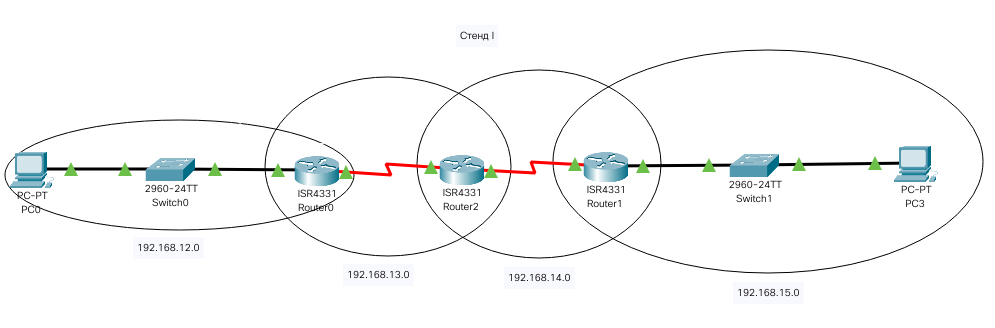
\includegraphics[scale=0.52]{img/1.png}
	\end{center}
	\caption{Разделение на подсети (первый стенд)}
	\label{fig:1}
\end{figure}

\begin{figure}[H]
	\begin{center}
		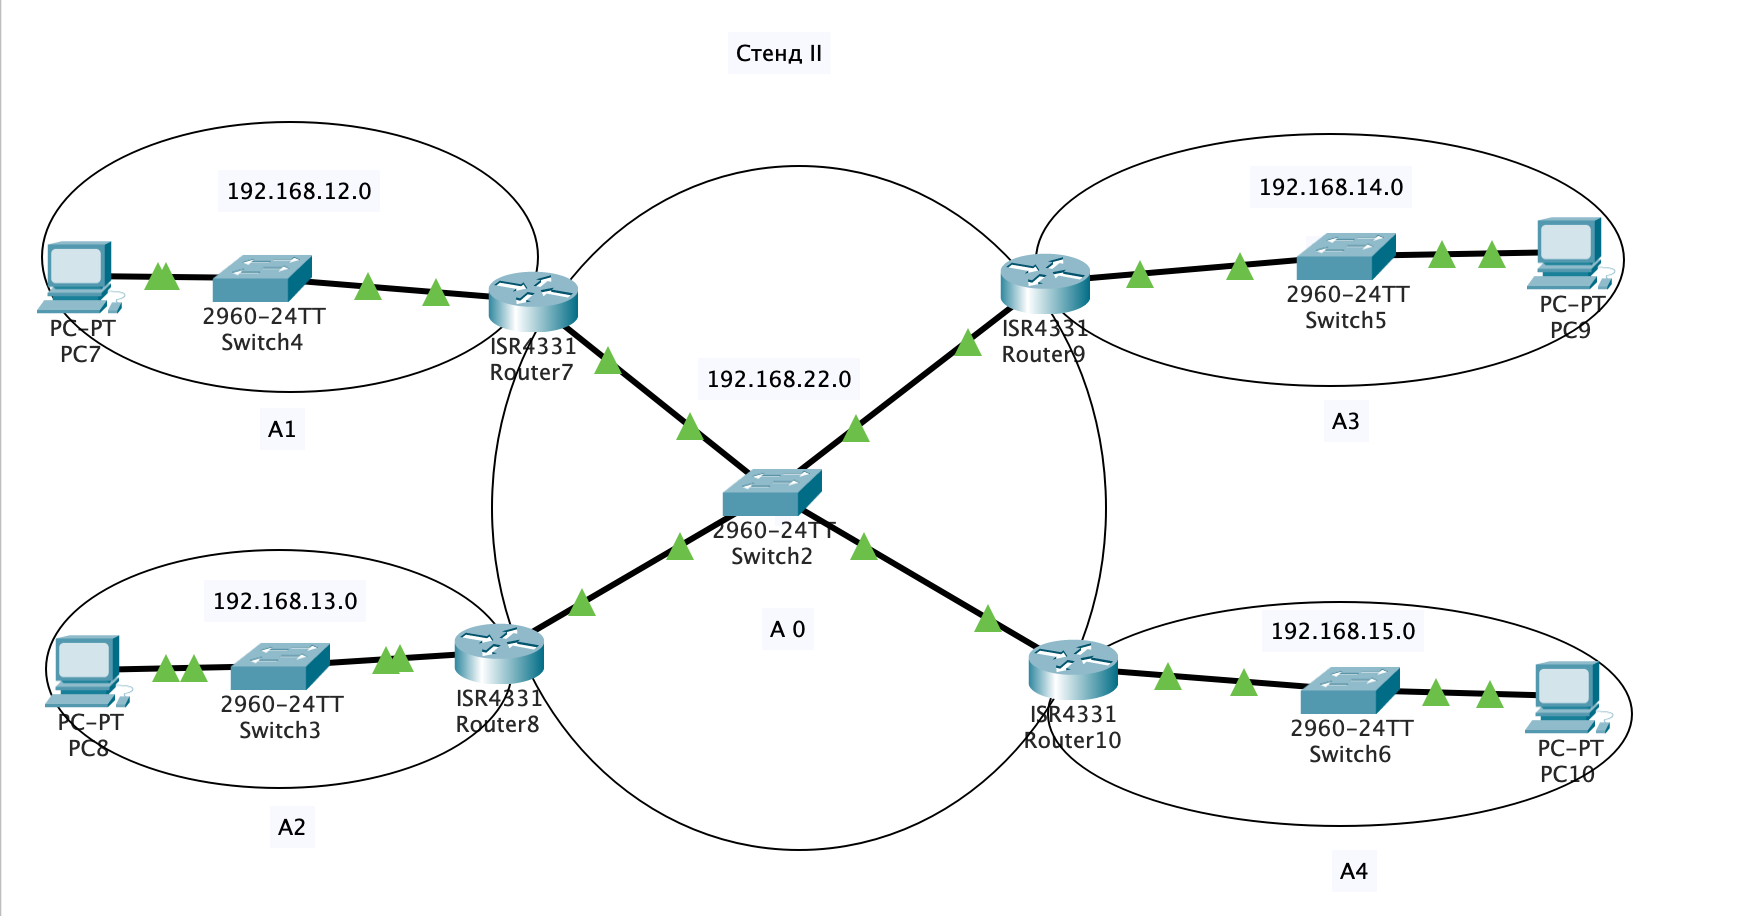
\includegraphics[scale=0.55]{img/2.png}
	\end{center}
	\caption{Разделение на подсети (второй стенд)}
	\label{fig:2}
\end{figure}

\subsection*{Настройка RIPv2}

На рисунке \ref{fig:3} представлены команды настройки Router0. Для остальных роутеров команды аналогичны.

\begin{figure}[H]
	\begin{center}
		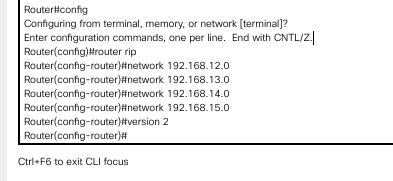
\includegraphics[scale=0.8]{img/3_1.png}
	\end{center}
	\caption{Настройка RIPv2 для Router0 (первый стенд)}
	\label{fig:3}
\end{figure}

\begin{figure}[H]
	\begin{center}
		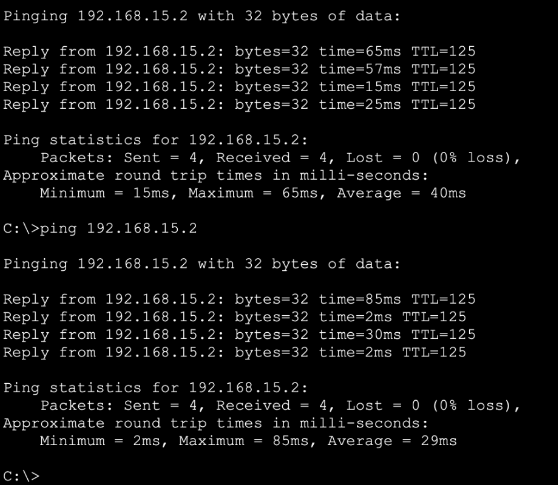
\includegraphics[scale=0.6]{img/4.png}
	\end{center}
	\caption{Проверка соединения между PC0 и PC3 с помощью команды \texttt{ping} (первый стенд)}
	\label{fig:4}
\end{figure}

\subsection*{Настройка OSPF}

На рисунках \ref{fig:5} - \ref{fig:8} представлены команды для настройки каждого из роутеров.

\begin{figure}[H]
	\begin{center}
		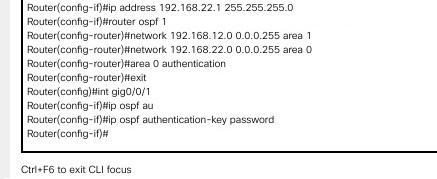
\includegraphics[scale=0.8]{img/5_1.jpg}
	\end{center}
	\caption{Настройка OSPF для Router7}
	\label{fig:5}
\end{figure}

\begin{figure}[H]
	\begin{center}
		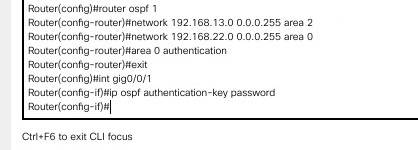
\includegraphics[scale=0.8]{img/6_1.jpg}
	\end{center}
	\caption{Настройка OSPF для Router8}
	\label{fig:6}
\end{figure}

\begin{figure}[H]
	\begin{center}
		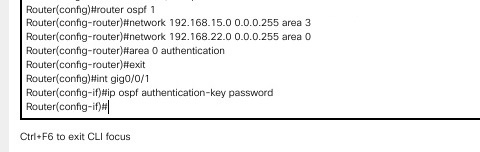
\includegraphics[scale=0.8]{img/7_1.jpg}
	\end{center}
	\caption{Настройка OSPF для Router9}
	\label{fig:7}
\end{figure}

\begin{figure}[H]
	\begin{center}
		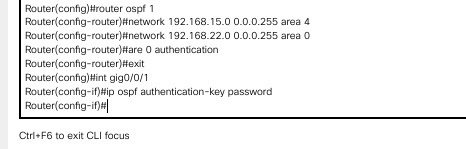
\includegraphics[scale=0.8]{img/8_1.jpg}
	\end{center}
	\caption{Настройка OSPF для Router10}
	\label{fig:8}
\end{figure}

На рисунке \ref{fig:9} представлен результат проверки статуса соседних устройств для Router8.

\begin{figure}[H]
	\begin{center}
		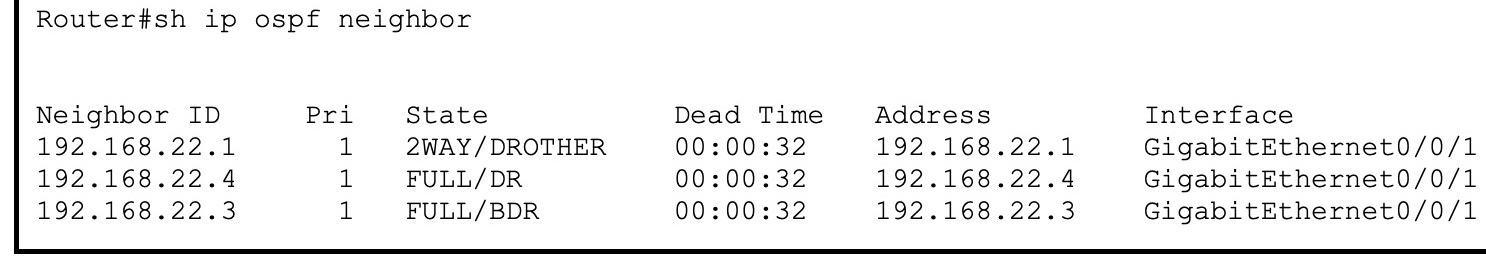
\includegraphics[scale=0.2]{img/9.jpg}
	\end{center}
	\caption{Статус соседних устройств для Router8}
	\label{fig:9}
\end{figure}

На рисунке \ref{fig:10} представлен результат проверки соединения между PC7 и PC10.

\begin{figure}[H]
	\begin{center}
		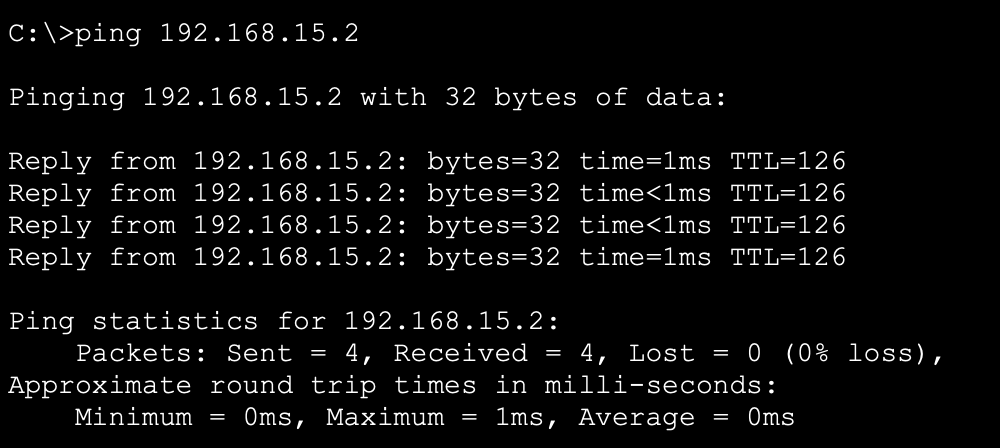
\includegraphics[scale=0.8]{img/10.png}
	\end{center}
	\caption{Проверка соединения между PC7 и PC10 с помощью команды \texttt{ping}}
	\label{fig:10}
\end{figure}

\bibliographystyle{utf8gost705u}
\bibliography{51-biblio}
	
\end{document}
